\documentclass[twocolumn]{article}
\usepackage{graphicx}
\usepackage{amsmath}
\usepackage{float}
\usepackage{amssymb} %Use of therefore symbol
\usepackage{hyperref}
\usepackage{caption}



\begin{document}
\title{Lab 1: Monte Carlo Methods}
\author{Alex Matheson, Austin Nhung}
%\affiliation{Department of Physics and Astronomy, University of Calgary, Calgary AB T2N 1N4 Canada}
\date{\today}
\maketitle

\section{Introduction}
Monte Carlo methods are a series of algorithms that take advantage of random processes to solve complicated systems. Many Monte Carlo methods are used to solve problems that are either difficult or impossible to solve analytically. This lab demonstrated a selection of Monte Carlo methods by applying them to simple mathematical and physical problems. Since all Monte Carlo methods rely on randomness, the lab first examined ways of defining randomness and evaluating simple pseudo-random number generators. Sampling and the metropolis algorithm were demonstrated in a simulation of photon transfer through a material. A simple Markov chain example involving meteorology was next considered. Lastly, the technique of annealing was used to demonstrate hill climbing and optimization. The examples in this lab showcases a number of Monte Carlo applications, but further applications include climate change simulations, radiation treatment, and financial planning.

\section{Methods}
\subsection{Random Numbers}
Fortran code was written to generate random numbers using a pseudo-random number generator, using input parameters $I_0=3$, $A=7$, $C=0$, and $M=10$. A number could then be generated by:

\begin{equation}
I_{n+1} = (AI_n + C) mod (M)
\end{equation} 

The sequence generated was shown to repeat, following a pattern of $1,7,9,3,...$ . This pattern was clearly not random due to its repetition. For this algorithm a given sequence must repeat after at most $M$ entries. Since there are $M$ possible results from the equation, the longest possible sequence generates each number $0=<n<M$ at most once, since once a previous value from the sequence is drawn, the sequence begins to repeat. 

A more elaborate version of this pseudo-random generator was constructed with larger constants. A correlation plot was made to visualize how subsequent values in the sequence were related. Figure \ref{fig:fig1} shows the plot, along with the parameters used to calculate it. The result showed that this sequence was not truly random, with some pattern existing between the subsequent numbers. While the numbers were uniform, their equal spacing showed they were not entirely random. Another correlation plot, figure \ref{fig:fig2}, showed a different set of parameters. The numbers in this sequence clearly followed a repeating pattern. In pseudo-random generators such as  the example here, the number of random numbers before repetition is $n <= M$. In this case, the less than nature is evident. Figure \ref{fig:fig3} shows a plot without such problems. The results in this case appeared to have no correlation between $x_n$ and $x_{n+1}$ and are shown similar to random noise. Still, other methods should be used to verify that there are no underlying patterns present. 

\begin{figure}[h]
\centering
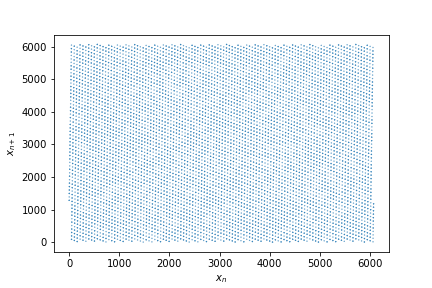
\includegraphics[width=\linewidth]{fig1}
\caption{A correlation plot for a pseudo-random sequence with $A=106$, $C=1283$, and $M=6075$.}
\label{fig:fig1}
\end{figure}

\begin{figure}[h]
	\centering
	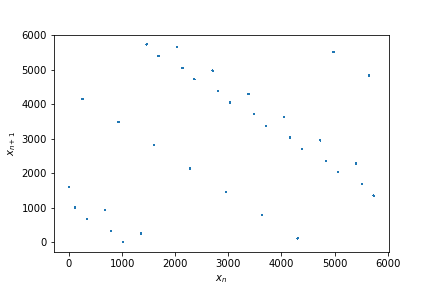
\includegraphics[width=\linewidth]{fig2}
	\caption{A correlation plot for a pseudo-random sequence with $A=107$, $C=1283$, and $M=6075$. Note that this is a change of 1 in variable $A$ from figure \ref{fig:fig2}}
	\label{fig:fig2}
\end{figure}

Next, the autocorrelation function was examined. It was defined according to equation 10 in the lab handout. A good sequence of random numbers should have a low autocorrelation value, indicating that numbers were independent from one another. The above pseudo-random generator was tested alongside the gfortran random number generator.

\begin{figure}[H]
	\centering
	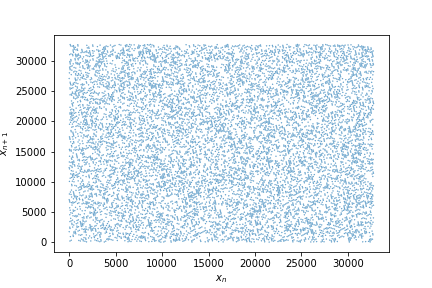
\includegraphics[width=\linewidth]{fig3}
	\caption{A correlation plot for a pseudo-random sequence with $A=1103515245$, $C=12345$, and $M=32768$.}
	\label{fig:fig3}
\end{figure}

As mentioned above, a correlation plot alone does not determine randomness. Figure \ref{fig:fig4} shows that values previously assumed to be random most certainly were not. When looking at the sequence of numbers generated, the top of the figure clearly showed a repeating pattern present. The autocorrelation function also showed that it takes some time for the auto-correlation to approach zero. 

The gfortran random number generator was also tested. The sequence of values obtained appears random to the naked eye. The auto-correlation plot also shows an expected decrease toward zero. The value of the auto-correlation function at its peak also was also approximately half that of the previous pseudo-random generator. As one would expect, the fortran's inherent generator was constructed better than a single line equation, both in terms of values generated, and auto-correlation.

\begin{figure}[h]
\centering
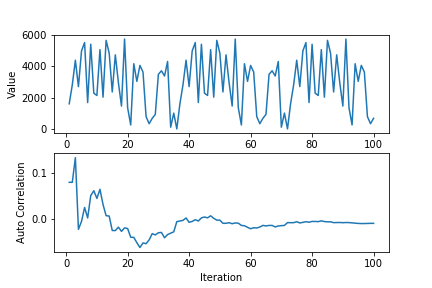
\includegraphics[width=\linewidth]{fig4}
\caption{Random numbers generated by the same pseudo-random generator as figure \ref{fig:fig3}. The top plot shows the numbers generated, while the bottom plot shows the auto-correlation function.}
\label{fig:fig4}
\end{figure}

\begin{figure}[h]
	\centering
	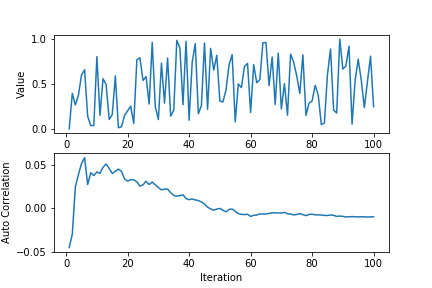
\includegraphics[width=\linewidth]{fig5}
	\caption{Random numbers generated by gfortran's internal RAND() function.}
	\label{fig:fig5}
\end{figure}

\subsection{Light Diffusion}
A number of equations were provided for different parameters in a light diffusion scenario. In this scenario, a photon enters a uniform slab and interacts with matter inside. The possible interactions are absorption, scattering, or exiting the medium. To simulate the path of a single photon through the slab, each parameter in the equations need to be randomly sampled. These parameters are not necessarily uniform. Using the fundamental principle, three sampling equations were determined. To di this, each probability density was turned into a cumulative probability density, and then inverted. The sampling equation for optical depth was determined below:

\begin{equation}
\label{eq:tau_sample}
\begin{split}
P(\tau) d\tau =& e^{-\tau} d\tau \\
F_{\tau} (\tau) =& \frac{\int_{0}^{x} e^{-\tau} d\tau}{\int_{0}^{\tau_{max} = 10} e^{-\tau} d\tau}\\
				=& \frac{-e^{-x} + 1}{-e^{-10} + 1}\\
\tau =& F^{-1}_{\tau}(u) \\
\tau =& -ln(1-u(1-e^{-10}))
\end{split}
\end{equation}

Next, the distribution for initial orientation $\theta$ was provided. From this random samples could be determined:
\begin{equation}
\label{eq:theta_sample}
\begin{split}
P(\theta) d\theta =& \frac{1}{2} \sin(\theta) \\
F_{\theta} (\theta) =& \frac{\int_{0}^{x} \frac{1}{2} sin(\theta) d\theta}{\int_{0}^{\pi} \frac{1}{2} sin(\theta) d\theta}\\
					=& \frac{-\cos(x) + 1}{2}\\
\theta =& F^{-1}_{\theta}(u) \\
\theta =& \arccos(1-2u)
\end{split}
\end{equation}

Lastly, angle $\phi$ needed to be considered. Thankfully, this variable was already uniform.

The length traveled through the medium was dependent on the optical depth. This may be defined using the following equations:
\begin{equation}
\tau = \int^L_0 n \sigma ds = n \sigma L
\end{equation}

\begin{equation}
\begin{split}
\tau &= \int n \sigma dz \\
\tau &= n \sigma z\\
\tau_{max} &= n \sigma z_{max} \\
\tau_{max} &= (\frac{\tau}{L}) z_{max} \\
L &= \frac{\tau z_{max}}{\tau_{max}}
\end{split}
\end{equation}
Hence, $L$ is the ratio of how far through the vertical thickness the photon has traveled.

When a photon reaches the end of a medium it will exit. For the rest of the medium, the photon may be scattered or absorbed. The probability of a photon being scattered is:
\begin{equation}
prob = \frac{P_s}{P_s + P_a}
\end{equation}

The $P_s$ and $P_a$ terms are the probability of scattering and absorbing respectively. The overall probability has two extreme cases. Since the two probabilities must add together to $1$, the absorb or scatter condition has value $1$ associated with complete scattering (when $P_s = 1$ and $P_a=0$) or value $0$ for complete absorption (when $P_s = 0$ and $P_a=1$).

To test the sampling distributions, each random number formula was written in fortran and used to generate a series of histograms. If the histograms recreated the original probability densities set out for the variable, the random generator was assumed to be working correctly. Figures \ref{fig:fig6}, \ref{fig:fig7} and \ref{fig:fig8} show $\tau$, $\theta$ and $\phi$ samples respectively.

\begin{figure}[t]
\centering
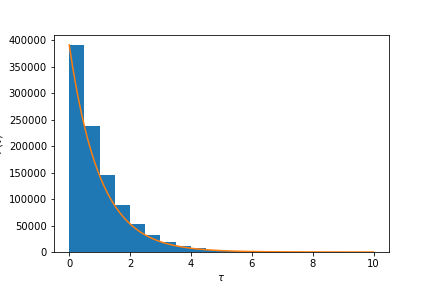
\includegraphics[width=\linewidth]{fig6}
\caption{Histogram for random values of $\tau$ generated by final equation \ref{eq:tau_sample}. The orange curve represents the expected distribution.}
\label{fig:fig6}
\end{figure}

\begin{figure}[t]
\centering
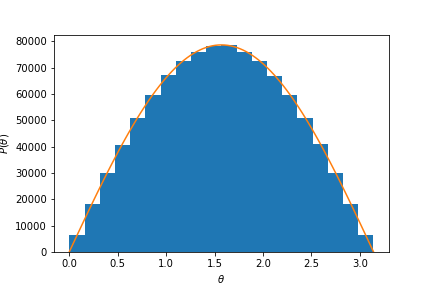
\includegraphics[width=\linewidth]{fig7}
\caption{Histogram for random values of $\theta$ generated by the final equation in set \ref{eq:theta_sample}. The orange curve represents the expected distribution}
\label{fig:fig7}
\end{figure}

\begin{figure}[h]
	\centering
	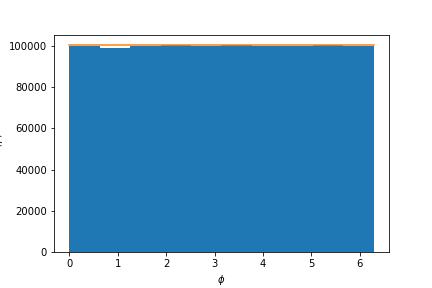
\includegraphics[width=\linewidth]{fig8}
	\caption{Histogram for random values of $\phi$ generated by a uniform random number generator. The orange curve represents the expected distribution.}
	\label{fig:fig8}
\end{figure}

Next, the simulation of a photon in a purely scattering medium was examined. The simulation was allowed to run for $10^6$ iterations. The exit angle of each exiting photon was plotted in figure \ref{fig:fig9}. Once this was completed, the fortran script converted the histogram data to intensity of light at the corresponding angle, using the equation 18 in the lab handout. The data were then plotted against the expected intensity values for this range of angles. Figure \ref{fig:fig10} shows the intensity of both experimental and theoretical light.

\begin{figure}[h]
\centering
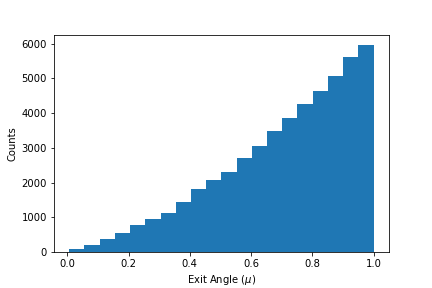
\includegraphics[width=1\linewidth]{fig9}
\caption{Histogram of exit angles for photons travelling through a purely scattering slab.}
\label{fig:fig9}
\end{figure}

\begin{figure}[h]
\centering
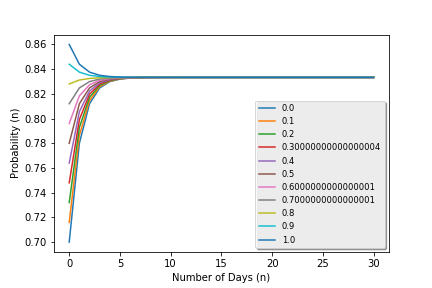
\includegraphics[width=1\linewidth]{fig10}
\caption{Intensity of light exiting a purely scattering slab. The blue line represents the data found by simulation. The orange line is the expected theoretical value for the same range. Note that the experimental data were binned into 20 bins, resulting in a jagged appearance compared to the higher resolution expected curve.}
\label{fig:fig10}
\end{figure}

A test case with the probability of absorption and scattering equal ($P_a=0.5$) was performed to simulate a more realistic case. The number of iterations had to be drastically higher ($10^9$), to account for the fact that many more photons were absorbed or reflected back out of the slab in this simulation. Figure \ref{fig:fig11} shows the histogram of different exit angles of photons exiting, whereas figure \ref{fig:fig12} shows the intensity.

\begin{figure}
\centering
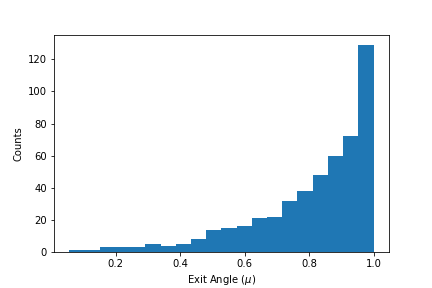
\includegraphics[width=\linewidth]{fig11}
\caption{Exit orientations of a slab that equally scatters and absorbs.}
\label{fig:fig11}
\end{figure}

\begin{figure}
\centering
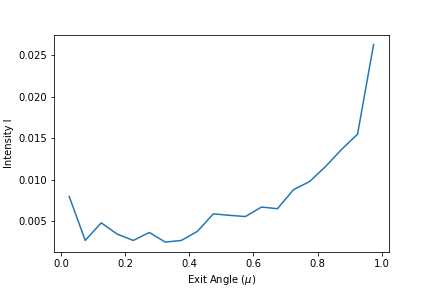
\includegraphics[width=\linewidth]{fig12}
\caption{The intensity of light emitted at different angles upon exit from an equally scattering and absorbing slab.}
\label{fig:fig12}
\end{figure}


\subsection{Markov Chain Monte Carlo}
To examine Markov Chain Monte Carlo, a simple meteorology problem was examined considering weather being rainy or sunny. The transition matrix for this problem was as follows:

\[ P = \begin{pmatrix}
	0.9 & 0.5 \\
	0.1 & 0.5
\end{pmatrix} \]

The transition matrix allowed predictions to be made once an input state for the system was provided. If the weather is sunny today, then for tomorrow:
\[ 
\begin{pmatrix} 0.9 & 0.5 \\ 0.1 & 0.5 \end{pmatrix} \begin{pmatrix} 1 \\ 0\end{pmatrix}
= \begin{pmatrix}0.9 \\ 0.1 \end{pmatrix}
\]

For two days from now:

\[
\begin{pmatrix} 0.9 & 0.5 \\ 0.1 & 0.5 \end{pmatrix} \begin{pmatrix} 0.9 & 0.5 \\ 0.1 & 0.5 \end{pmatrix} \begin{pmatrix} 1 \\ 0\end{pmatrix}
=
\begin{pmatrix} 0.86 \\ 0.14\end{pmatrix}
\]

Over time, a Markov chain should reach an equilibrium. To verify, the probability of sunny and rainy weather was forecast up to 100 days in the future. A fortran program was written to multiply the previous day's forecase with the transition matrix. Figure \ref{fig:fig13} shows the forecast starting from both a sunny and rainy day.

\begin{figure}
\centering
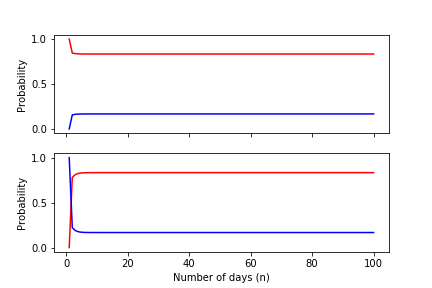
\includegraphics[width=\linewidth]{fig13}
\caption{Plots of probabilities of future weather. The upper plot starts from a sunny day and the lower plot from a rainy day. The blue line is the probability of a day being rainy, and the red of a day being sunny. In both cases the forcast reaches the same equilibrium.}
\label{fig:fig13}
\end{figure}

Well before 100 days, the system in both cases reaches an equilibrium. The matrix below was determined by running a matrix multiplying fortran code over 100 iterations, with the matrix below as the result. All entries involved repeating decimals to 6 decimal places. It was assumed that the values would be infinitely repeating if it were not for machine error. This was verified in a later analytic solution.
\[ P^{100} = \begin{pmatrix}
0.8\bar{3} & 0.8\bar{3} \\
0.1\bar{6} & 0.1\bar{6}
\end{pmatrix} \]

In general, Markov chain equilibrium may be solved by a series of equations. In this case:
\begin{equation}
\begin{split}
p_{sun} &= 0.9 p_{sun} + 0.5 p_{rain} \\
p_{rain} &= 0.1 p_{sun} + 0.5 p_{rain} \\
p_{sun} &+ p_{rain} = 1
\end{split}
\end{equation}

These may be solved analytically to yield:
\begin{equation}
\begin{pmatrix} p_{sun} \\ p_{rain} \end{pmatrix}
= \begin{pmatrix} 5/6 \\ 1/6 \end{pmatrix}
\end{equation}

Which matches the above findings.

Lastly, it was demonstrated that no matter the starting situation, this same equilibrium was the end result. To demonstrate this, an extreme case was used where days could assume decimal values for the sunny and rainy states, as long as both indices of the current-day vector summed to one. Figure \ref{fig:fig14} shows the outcome of this test. In all cases, the same equilibrium was obtained.

\begin{figure}
\centering
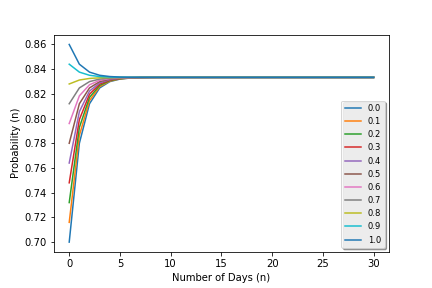
\includegraphics[width=\linewidth]{fig14}
\caption{Probability of a day n days into the future being sunny. Each coloured line represents a different starting state. In this example the extreme case of a day being a fraction sunny and having a starting vector with decimal places. In all cases, the equilibrium is the same.}
\label{fig:fig14}
\end{figure}

\subsection{Metropolis-Hastings}
The Metropolis-Hastings algorithm is a variation of the Metropolis algorithm, so
to explore this idea, a simple Metropolis random-walk is simulated. The big idea
behind the Metropolis algorithm is creating ``walkers'' which travel through the
probability space, and the walkers approach the correct probability distribution
after a large number of steps. The main difference between Metropolis and
Metropolis-Hastings is the addition of a proposal distribution from which the
direction and size of each step is sampled from. The proposal distribution can
be symmetrical, as is in the case of Metropolis, or asymmetrical, as it is in
Metropolis-Hastings.

Each step is given a weight, defined as
\begin{equation}
	\alpha(x') = \min \left( 1, \frac{p(x') q(x' | x)}{p(x) q(x | x')} \right)
	\label{eq:acceptance}
\end{equation}
where $p$ is the target distribution, $q$ is the proposal distribution, and $x'$
is the proposed step from $x$. This weighting forces steps toward a local
maximum to always be accepted, but steps away from the local maximum are
accepted with some probability. The state-to-state process describes a Markov
chain, which was explored earlier. Another consequence of this weighting is that
neither the target distribution nor the proposal distribution need to be
normalized. This property can be very advantageous when sampling a complicated
distribution.

For a simple example, we consider the target distribution
\begin{equation}
	P(x) = \frac{1}{2 \sqrt{2}} \left( \sin(5x) + \sin(2x) + 2 \right) e^{-x^2}
	\label{eq:example}
\end{equation}
and the proposal distribution
\begin{equation}
	q(x | x') = \frac{1}{\sqrt{2 \pi \sigma^2}} \exp \left( - \frac{(x' - x)^2}{2 \sigma^2} \right)
\end{equation}
Since the normal distribution is symmetrical, this is actually equivalent to
distribution which moves in the opposite direction, from $x'$ to $x$, since the
square term in the exponential can be reversed. Thus, for the normal
distribution,
\begin{equation}
	q(x | x') = q(x' | x)
\end{equation}

The acceptance probability from \ref{eq:acceptance} is then reduced to
\begin{equation}
	\alpha(x') = \min \left( 1, \frac{p(x')}{p(x)} \right)
\end{equation}
This returns the acceptance probability of the simple Metropolis algorithm. The
intuitive reason why the ratio of proposal distributions disappears is that the
ratio describes the relative probability of moving one way, from $x$ to $x'$,
versus the other. The reason this ratio is included is to give greater control
over how the walkers traverse the probability space. The motivation to seek
greater control is to avoid completely relying on the target distribution, where
the walkers may get trapped in a local maxima. The problem is more daunting as
the number of degrees of freedom increases, leading to the curse of
dimensionality.

Once the acceptance probability of a proposed step is calculated, a random
number $r$ from a uniform distribution is generated, and the step is accepted
with the probabilities
\begin{equation}
	x_{n+1} = \left\{
	\begin{array}{lr}
		x', & \text{if} \, r <= \alpha(x') \\
		x_n & \text{if} \, r > \alpha(x')
	\end{array}
	\right.
\end{equation}

Continuing on with the example distribution \ref{eq:example}, the
Metropolis-Hastings algorithm was implemented with three different values for
standard deviation $\sigma = 0.025, 1.0, 50$ in order to compare the effects of
using a very narrow or very wide proposal distribution. As shown in figure
\ref{fig:mcmc1}, a very narrow distribution confines the walkers to a limited
space. The walkers will traverse the probability space much more slowly, and
there is a greater chance of staying at a local maxima rather than exploring the
entire space. This is the reason the narrow proposal distribution remains around
$x = -1$. The wide distribution is the opposite and is able to explore the
entire probability space. However, as the bottom half of figure \ref{fig:mcmc1}
shows, the walker was also very likely to reject steps and remained stagnant for
longer periods of time. A suitably chosen proposal distribution is very
important for getting an accurate result.

\begin{figure}[p]
	\centering
	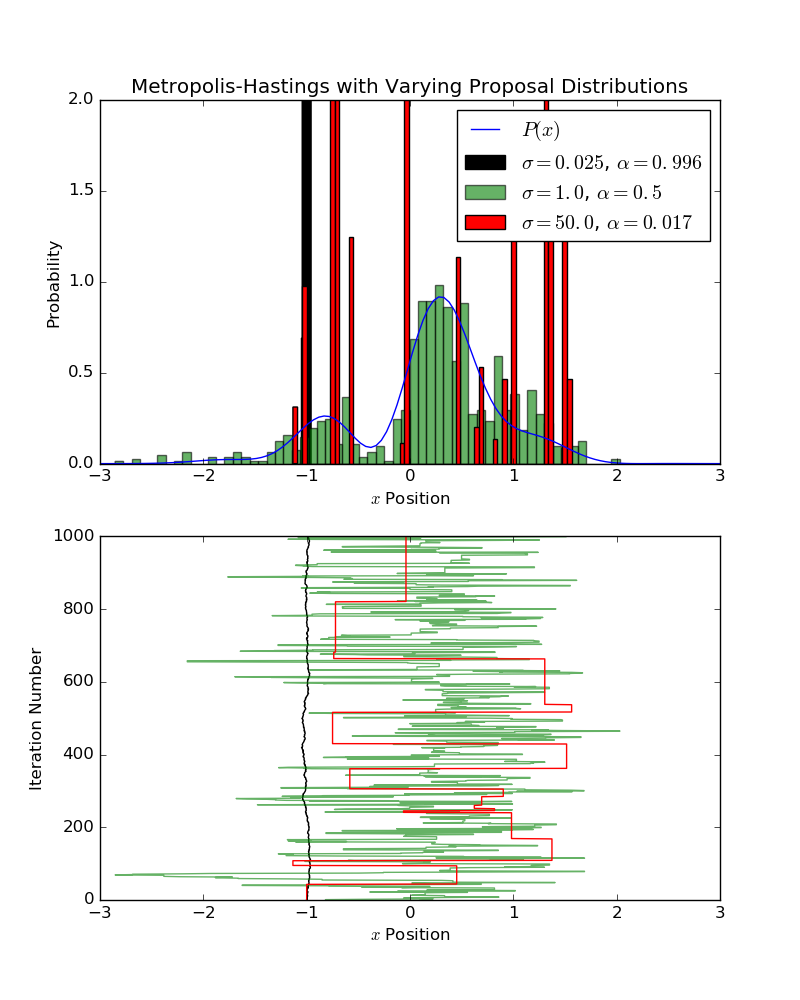
\includegraphics[width=\linewidth]{mcmc1.png}
	\caption{
		The Metropolis-Hastings algorithm was used to sample the probability space
		of equation \ref{eq:example} with a normal proposal distribution, run for
		$1\,000$ steps. The width of the proposal distribution was varied, where
		$\sigma$ is the standard deviation, and $\alpha$ is the acceptance rate. The
		top half shows the resulting probability distribution by taking the
		histogram of the random walk, as well as the true distribution $P(x)$. The
		bottom half shows the Markov chain and the position of each walker over
		time.
	}
	\label{fig:mcmc1}
\end{figure}

The program used in figure \ref{fig:mcmc1} was only run for $1000$ steps, and
the law of large numbers states that the random walk should approach the correct
distribution given a large number of steps. To test this, we ran the same
program again with $50\,000$ steps, shown in figure \ref{fig:mcmc2}. As
predicted, the results for the very narrow and very wide proposal distributions
improved over time. However, it should be noted that with a very small $\sigma$,
the walker was only able to explore the area around the local maxima where it
started. The walker with very large $\sigma$ still has a very low acceptance
rate, and the result is oversampling the global maxima. On the other hand, the
reasonably chosen $\sigma$ has a very good fit under the curve, which has only
improved over time.

\begin{figure}[p]
	\centering
	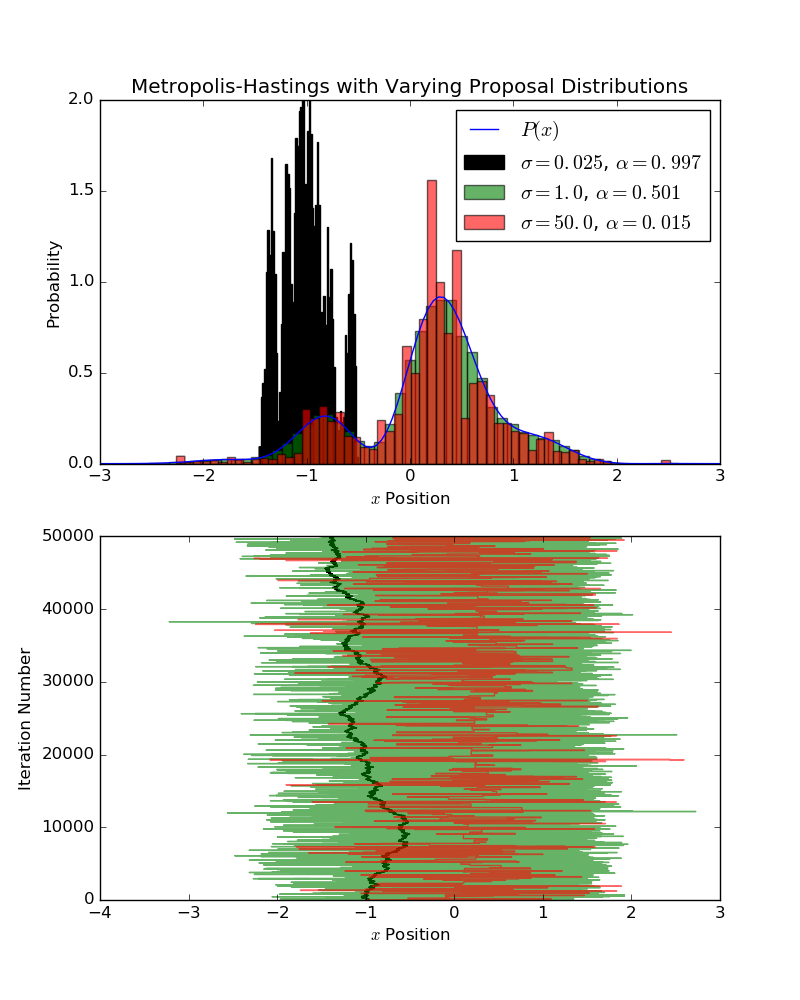
\includegraphics[width=\linewidth]{mcmc2.png}
	\caption{
		The Metropolis-Hastings algorithm was used in the same way as in figure
		\ref{fig:mcmc1} but with $50\,000$ steps. No other parameters were changed.
	}
	\label{fig:mcmc2}
\end{figure}

The burn-in phase refers to the process of the walkers moving toward an
equilibrium. The number of steps this takes is highly dependent on the choice of
starting values and how suitable the proposal distribution is. This time, all
parameters will be kept the same, so the walkers all start at $x_0 = -3$,
$\sigma = 0.2$, and are all run for $1\,000$ steps. The difference between the
two experiments is only the distribution done at the end, where in figure
\ref{fig:burn1} all steps are kept as the control case and \ref{fig:burn2} is
the experiment with burn-in, and the first $200$ steps are discarded.

\begin{figure}[p]
	\centering
	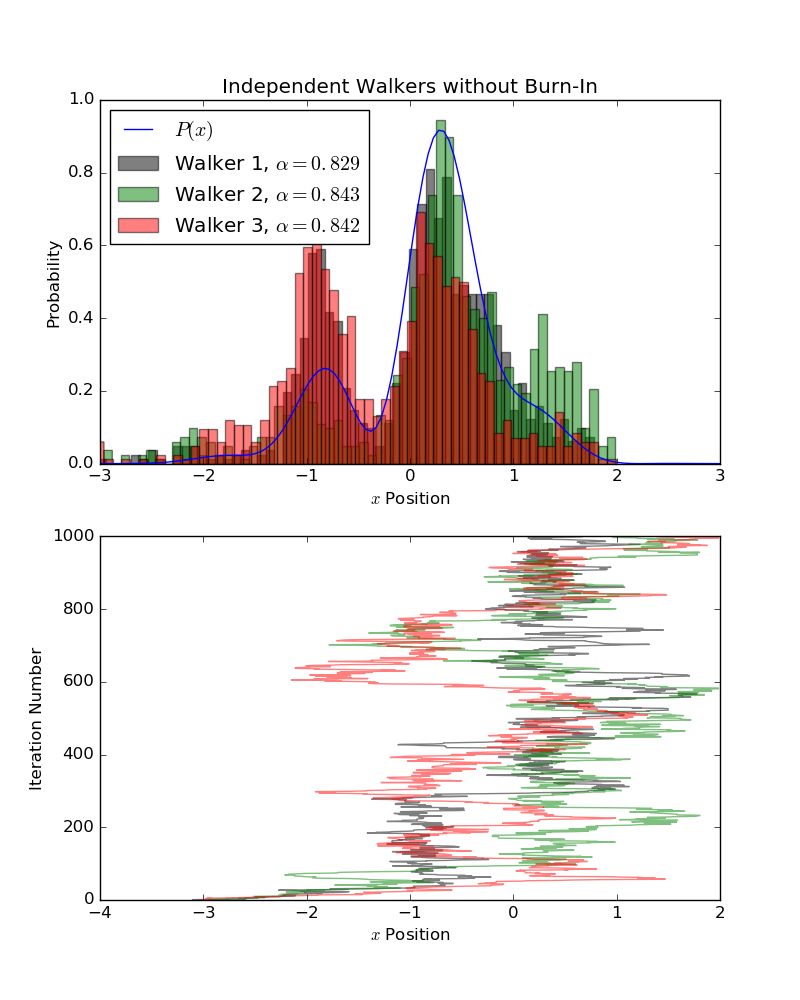
\includegraphics[width=\linewidth]{burn1.png}
	\caption{
		The Metropolis-Hastings random-walk for three identitcal walkers, starting
		at $x_0 = -3$, standard deviation $\sigma = 0.2$, and run for $1\,000$
		steps. This is the control case where all steps are kept. This is to compare
		with figure \ref{fig:burn2} where the burn-in phase is considered.
	}
	\label{fig:burn1}
\end{figure}

\begin{figure}[p]
	\centering
	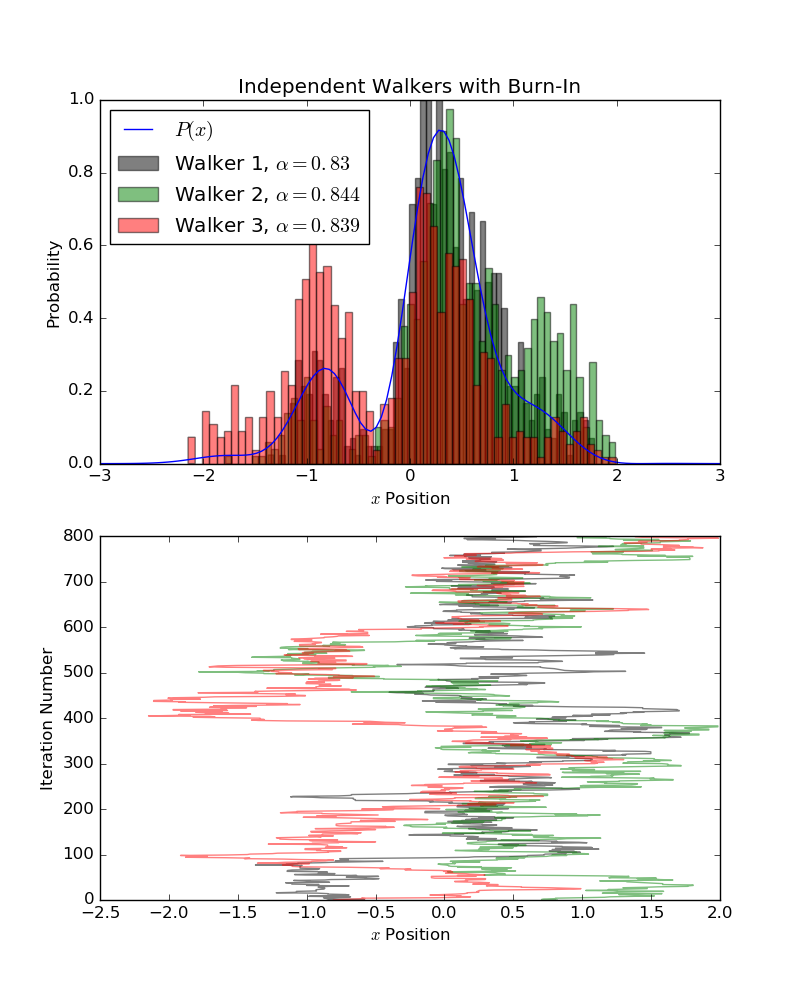
\includegraphics[width=\linewidth]{burn2.png}
	\caption{
		The Metropolis-Hastings random-walk with burn-in phase considered. The first
		$200$ of $1\,000$ steps were discarded. Since this was run with identical
		conditions as it was in figure \ref{fig:burn1}, the walks are very similar
		since the same seed was used. The only difference is which steps were
		discarded or kept.
	}
	\label{fig:burn2}
\end{figure}

By comparing figure \ref{fig:burn1} with figure \ref{fig:burn2}, the most
obvious difference is how the experiment that considers the burn-in phase can
avoid oversampling the local maxima centered around $x = -1$. The reason the
oversampling occurs in the first place is the walkers began at the edge of the
distribution, far away from the center of the distribution. This is not always a
problem very easily solved, and is improved by allowing the system to reach a
state closer to equilibrium before we begin considering every step.


\subsection{Annealing}
In an annealing procedure, the acceptance probability of completing a change after a proposed step forward is modified by a temperature $T$. The acceptance is now defined as:
\begin{equation}
A(x_n \to x^*) = Min \Bigg( 1, \Big( \frac{P(x^*)}{P(x_n)}\Big) ^{ \frac{1}{T(n)} } \Bigg)
\end{equation}
When $T=1$, the algorithm that is recovered is a simple metropolis algorithm. 

In a hypothetical scenario, the probability term is set to 0.5 and $T=100$ initially, yielding acceptance of $0.93$. After some time, $T=1$ and the acceptance reduces to $0.5$. After still more time, $T=0.1$ and the acceptance is $0.000977$. Because of the inverse nature of $T$ in the exponent, a reduction in $T$ makes a change exponentially less likely to occur. This is typically desirable when using annealing. Ideally, the random walker being used by the algorithm is able to escape local maxima and jump to other peaks in the region early on. As time goes on, the algorithm should lower the acceptance so that it hones in on the actual peak.

In another hypothetical scenario, the probability density of a system is $P(x) = e^{-E}$. For such a system, the acceptance is as follows:
\begin{equation}
\begin{split}
A(x_n \to x^*) =& Min \Bigg( 1, \Big( \frac{P(x^*)}{P(x_n)}\Big) ^{ \frac{1}{T(n)} } \Bigg) \\
A(x_n \to x^*) =& Min \Bigg( 1, \Big( \frac{e^(-x^*)}{e^-x_n}\Big) ^{ \frac{1}{T(n)} } \Bigg) \\ 
A(x_n \to x^*) =& Min \Bigg( 1, e^{\frac{-(x^* - x_n)}{T(n)}} \Bigg)
\end{split}
\end{equation}
This looks like a decay equation, found in many areas of physics. For instance, this could describe a decaying wave function. Likewise, this shares similarities to a nuclear decay equation.

\subsection{Hill Climbing}
One application of annealing is to finding minima and maxima, otherwise known as hill climbing. For this course, a sample presentation on hill climbing, including a written class, was given to the class. This code was modified to fit the examples provided in the lab. According to the code, a geometric temperature schedule was used according to:
\begin{equation}
T(t) = T_i * \bigg( \frac{T_f}{T_i} \bigg)^{(t/N)}
\end{equation}
 Where $T$ was the temperature, $t$ the time, $T_i$ the initial temperature, $T_f$ the final temperature, and $N$ the number of iterations to perform. Three different functions were provided, in order to determine their global maxima. The functions were:
\begin{equation}
\begin{split}
f_1(x,y) =& e^{-(x^2+y^2)} \\
f_2(x,y) =& e^{-x^2+y^2} + 2e^{-[(x-1.7)^2 + (y-1.7)^2]} \\
f_3(x,y) =& (1-x)^2 + 100(y-x^2)^2
\end{split}
\end{equation}

In order to provide a visual check on the systems, as well as to get a general guess of the neighborhood of the minima and maxima, the three functions were plotted. Figures \ref{fig:function1}, \ref{fig:function2} and \ref{fig:function3} show each of the three functions, respectively.

\begin{figure}
\centering
\includegraphics[width=\linewidth]{"function 1"}
\caption{Visualization of function 1.}
\label{fig:function1}
\end{figure}

\begin{figure}
	\centering
	\includegraphics[width=\linewidth]{"function 2"}
	\caption{Visualization of function 2.}
	\label{fig:function2}
\end{figure}

\begin{figure}
	\centering
	\includegraphics[width=\linewidth]{"function 3"}
	\caption{Visualization of function 3.}
	\label{fig:function3}
\end{figure}

Figures \ref{fig:figure1maximum}, \ref{fig:figure2maximum}, \ref{fig:figure3maximum} show histograms of the x and y coordinates where the code determines a maxima is located. Both function 1 and 2 produced a definitive result, with a high peak near the mean of the histogram data. Function 3 however, was much less conclusive. Both x and y coordinates, had the 'best results' at very high values. This can be compared to the visualization of the function in figure \ref{fig:function3}. Running the hill climbing algorithm on function 3 produced a very narrow distribution for a minimum centred at $x=1.0006$, and $y=1.0004$. This suggested a peak at (1,1). 

The time to evaluate all three functions was tracked using the python time library and was shown in table \ref{tab}. Function 2 was the longest to evaluate, taking approximately $35s$ longer than the other two functions.

\begin{table}
\begin{center}
\begin{tabular}{|c|c|}
	\hline Function & Time \\ 
	\hline Function 1 & $93.2s$  \\ 
	\hline Function 2 &  $128.2s$\\ 
	\hline Function 3 & $94.4s$  \\
	\hline
\end{tabular} 
\caption{Evaluation time to find minimum or maximum of a given function.}
\label{tab}
\end{center}
\end{table}

\begin{figure}[p]
\centering
\includegraphics[width=\linewidth]{"figure 1 maximum"}
\caption{Histogram of found maxima for 1000 runs of a temperature controlled hill climb using function 1. The two plots show the distribution of x-coordinates of the final maximum on the left, and the y coordinate on the right. The maximum corresponds to a coordinate of approximately (0,0).}
\label{fig:figure1maximum}
\end{figure}

\begin{figure}[p]
	\centering
	\includegraphics[width=\linewidth]{"function 2 maximum"}
	\caption{Histogram of found maxima for 1000 runs of a temperature controlled hill climb using function 2. The two plots show the distribution of x-coordinates of the final maximum on the left, and the y coordinate on the right. The maximum corresponds to a coordinate of approximately (1.7,1.7).}
	\label{fig:figure2maximum}
\end{figure}

\begin{figure}[h]
	\centering
	\includegraphics[width=\linewidth]{"function 3 maximum"}
	\caption{Histogram of minima found for function 3 using a hill climb algoritm 1000 times. The two plots show the distribution of x-coordinates of the final minimum on the left, and the y coordinate on the right. The median of this distribution, corresponding to the minimum, was approximately (1,1).}
	\label{fig:figure3maximum}
\end{figure}



\section{Discussion}
The creation of random numbers is essential to the successful operation of Monte Carlo algorithms. The pseudo-random generator examined in this lab showed that its performance was extremely sensitive to initial parameters. The number of parameters generated is limited to a maximum of $M$, while the other parameters may produce conditions where fewer numbers are generated. Once a sequence of sufficient length was constructed, the results were not guaranteed to be random. Correlation plotting proved to eliminate certain parameters, however it also sometimes showed that a series was random, when other methods would disagree. Auto-correlation was also used to show how series entries were related to values further down the sequence. In all, the pseudo-random generator was extremely limited. It required very careful selection of parameters. Even if an ideal set of parameters was found, the series would always generate in the same order. A positive of the pseudo-random generator was its speed. When compared to the compiler, it was apparent that gfortran used a better, more sophisticated method than the pseudo-random sequence. 

Light diffusion was used as an example to demonstrate simple sampling routines based off the fundamental principle. As expected, coding using the inverse of cumulative density functions produced distributions of samples that matched the original probability density function. Two different examples were tested, a purely scattering slab and a slab with equal opportunity to absorb or scatter. For the scattering slab, the resulting output largely matched the theory. There was some variation from the theory nearer to $\mu=0$. With so few photons being emitted near these angles, a few extra photons may have been emitted at these levels due to the randomness of the simulation. Since the intensity at an angle is also proportional to the inverse of $\mu$, a few extra photons in a low angle bin would be amplified by the low $\mu$. The equal scattering / absorbing slab emitted fewer photons at low $\mu$. This was likely because photons exiting at a high angle were more likely to have traveled straight through, whereas moving through at angles would take a longer total path, increase the chance the photon would be absorbed.

Markov chains were examined using matrices and coding a markov chain algorithm in fortran. The expected equilibrium behavior was displayed. Furthermore, the results obtained through code were within machine error of the analytical values. A method was used that assumed daily weather could be a superposition of sun and rain. It was shown in all cases that the equilibrium condition is recovered, and the equilibrium value is the same for all starting states.

The Metropolis-Hastings algorithm is a special variant of the Metropolis algorithm used to sample probability spaces. Over time, these samplings approached the actual distribution of the space. The Metropolis-Hastings algorithm added a proposal distribution to describe how a random walker moved through the probability space, and provide restrictions on movement to fit a problem. For instance, a proposal distribution can specify if a walker favours one direction over another, or if the walker should take large or small steps. In the case of the pure metropolis algorithm, a normal proposal distribution results in a symmetry between opposite proposal distributions, eliminating the effect of the proposal distribution on the choice of whether or not to accept a move. 

Choosing an appropriate proposal distribution had a noticeable effect on the results of walkers. If a normal distribution was too narrow, the walkers did not sample the space effectively. If the distribution was too wide, computing resources were wasted with a large amount of rejected moves. It appears cleat that part of setting up a Monte Carlo problem is choosing an appropriate distribution that samples a space at a balance between completeness and efficiency. Burn in was another parameter to consider when designing a Monte Carlo problem. If insufficient burn in was used, the walker distribution was skewed. However, waiting too long for burn-in would waste computing resources. Clearly burn in also requires balance to ensure sampling begins as closely as possible to equilibrium.

Annealing was a method that was a modification of the Metropolis algorithm, designed to make the algorithm 'hone in' over  time. Different temperature regimes are possible, allowing one to control the rate at which the system becomes more selective. In the case of this lab, a geometric temperature scale was used. All three example functions had a minimum or maximum found which appeared to agree with visualizations of the function. Function 3 had a distribution of minimum coordinates that was far more spread out than those of functions 1 and 2. This may be due to the much lower gradient around function 3's minimum, compared to the two Gaussian maxima in functions 2 and 3. Because the gradient is so low, more movement is permitted in these regions at a given temperature than in the other functions. Of the three functions, 1 and 3 took roughly the same time to compute, whereas function 2 took much longer. This may be due to the complexity of function 2. Function 2 contained more calls to the natural exponent function, as well as a number of regular exponent calls, compared to the other two, so it stands to reason it would take longer.
 
\section{Conclusion}
Monte Carlo methods form a cornucopia of options when simulating complex systems computationally. As this lab has shown, they have the ability to sample, forecast, and optimize. At first glance, Monte Carlo methods appear to be a brute-force tool, simply doing the same thing over and over to approach a complex analytical problem. This lab has shown this to not be the case. Monte Carlo methods require careful tuning to ensure that the simulation matches reality closely, and that computations are solvable in a reasonable amount of time. This requires careful selection not only of the type of Monte Carlo method to best match the problem, but the selection of appropriate parameters as well. Parameters such as 'true' random numbers, proposal distributions, burn-in and cost functions can work to make solutions more efficient, more accurate, and more swift. While Monte Carlo may be a random method, the tools behind it are anything but.


\begin{thebibliography}{00}
	\bibitem{ouyed}
	Ouyed and Dobler, PHYS 581 course notes, Department of Physics and Astrophysics, University of Calgary (2016).
	\bibitem{NR}
	W. Press et al., \emph{Numerical Recipes} (Cambridge University Press, 2010) 2nd. Ed.
	\bibitem{Code}
	C. Hass and J. Burniston, MCMC Hill Climbing. Jupyter notebook, 2018.
\end{thebibliography}

\section{Appendix}
For access to the source codes used in this project, please visit \url{https://github.com/Tsintsuntsini/PHYS_581} for a list of files and times of most recent update.
	
\end{document}